\subsection{Light and Polarisation}

\subsubsection{Elliptic Polarisation Wave}\label{EllipticPolarisationWave}

The first good piece of news is that the magnetic part will not contribute, so less computation required. And we have the wave propagating in the $z$-direction.

\textbf{1):}

To show that $\vec{E}(0,t)$ parametrises an ellipse we just have to massage the given field components into:

\begin{equation}
	\begin{split}
		E_{x}(0,t)&= A \cos (-\omega t),\\
		E_{y}(0,t) & = B \cos (\phi - \omega t).
	\end{split}
\end{equation}

We also know that an ellipse looks like:

\begin{equation}\label{ellipseequation}
	a\: x^{2} + 2\: b\: xy + c \: y^{2} + f =0, \quad \quad \forall \: a,b,c,f \: \epsilon \quad \mathbf{R}_{+}.
\end{equation}

In this case, it is easy to think of both electric components as the $x,y$ components of the ellipse. Let's square them to rewrite \ref{ellipseequation}.

\begin{equation}
	\begin{split}
		E_{x}^{2}(0,t)&= A^{2} \cos^{2} (\omega t),\\
		E_{y}(0,t) & = B^{2} \cos^{2} (\phi - \omega t).
	\end{split}
\end{equation}

And now we prepare ourselves for a long boring trigonometrical computation\footnote{Recall to use trigonometrical identities to simplify!}. We start from:

\begin{equation}\label{EllipseMassage}
	\begin{split}
		&a \: E_{x}^{2} + 2\: b\: E_{y}\: E_{x} + c \: E_{y}^{2} +f =0,\\
		&\left(\underbrace{a \: A^{2} + 2 \: b \: A \: B \: \cos(\phi) + c \: B^{2} \: \cos^{2}(\phi)}_{\hat{A}}\right) \: \underbrace{\cos^{2} (\omega t)}_{x^{2}} +\\
		+& \left(\underbrace{c \: B^{2} \sin^{2}(\phi)}_{\hat{C}}\right)\: \underbrace{\sin^{2} (\omega t)}_{y^{2}} +\\
		+& \left(\underbrace{2 \: b \: A \: B \sin(\phi) + 2 \: c \: B^{2} \cos(\phi) \sin(\phi)}_{\hat{B}}\right)\: \underbrace{\cos (\omega t) \sin (\omega t)}_{x \: y} + f =0.
	\end{split}
\end{equation}

Where we have done all those identifications to mimic an ellipse equation. We are almost there. The main problem right now is that $\hat{A},\hat{B},\hat{C}$ have a dependence on $\phi$. This means that they are not fixed and the appearance of the ellipse is not defined in the form of a circle. We have to fix those values.

How do we get a circle? In this case we have $\hat{B} = 0, \hat{A}= \hat{C}$ so the equation results into $x^{2} + y^{2} + \tfrac{f}{a} = 0$. The first and and most natural thought is to set $\phi  = 0$, which makes $\hat{B} =0 $ but not $\hat{C}$... So we need something more involved, of the form:

\begin{equation}\label{Bcondition}
	\begin{split}
		\hat{B} &= \left(\underbrace{2 \: b \: A \: B  + 2 \: c \: B^{2} \cos(\phi)}_{0}\right) \sin (\phi) \rightarrow \\
		 &\rightarrow \: b \: A \: B = - \: c \: B^{2} \cos(\phi).
	\end{split}
\end{equation}

We also need:
	
\begin{equation}\label{ACcondition}
	\begin{split}
		& \underbrace{a \: A^{2} + 2 \: b \: A \: B \: \cos(\phi) + c \: B^{2} \: \cos^{2}(\phi)}_{\hat{A}} = \underbrace{c \: B^{2} \sin^{2}(\phi)}_{\hat{C}},\\
		& \rightarrow \quad \text{substitute \ref{Bcondition} and compute trigonometrics} \rightarrow\\
		& a \: A^{2} = c \: B^{2}.
	\end{split}
\end{equation}

Then, with \ref{Bcondition} and \ref{ACcondition} in mind, we go back to \ref{EllipseMassage} to determine $f$ as:

\begin{equation}\label{fcondition}
	f = - a^{2}\: A^{2} \: \sin^{2}(\phi).
\end{equation}

With all previous requirements we have a parametrisation of a circle as desired.
	
\textbf{2):}

Well, well, this part of the exercise looks like we have to change the basis of our system. The current description of the electric field is given by:

\begin{equation}\label{oldfield}
	\mathbf{E}(\vec{x},t) = \left(A \cos (kz - \omega t), B \cos (kz - \omega t + \phi) , 0\right).
\end{equation}

That we have to transform into something of the form:

\begin{equation}\label{newfield}
	\mathbf{E}_{\pm}(\vec{x},t)_{New} = \Re \left[\mathbf{E}_{+}(z,t) + \mathbf{E}_{-}(z,t)\right].
\end{equation}

And we know how the electric field looks like in this new basis as:

\begin{equation}
	\mathbf{E}_{\pm} = \tfrac{A_{\pm}}{\sqrt{2}}(\hat{x}\pm i \hat{y})e^{i(kz - \omega t)}.
\end{equation}

So it seems that the only thing we have to do is to sum to prove that (\ref{newfield}) is exactly the same as (\ref{oldfield}). Then:

\begin{equation}
	\begin{split}
		\Re \left[\mathbf{E}_{+} + \mathbf{E}_{-}\right]&= \Re\left[\left(\underbrace{\tfrac{A_{+}+ A_{-}}{\sqrt{2}}}_{A} e^{i \cdots} \hat{x} + \underbrace{\tfrac{i(A_{+}- A_{-})}{\sqrt{2}}}_{B} e^{i \cdots} \hat{y}\right)\right] =\\
		&= \Re \left[A e^{i \cdots} \hat{x} + B e^{i \cdots} \hat{y} \right] =\\
		&= \text{Expand with} \: e^{i x} = \cos x + i \sin x \: \text{and let $\Re$ kill the imaginary terms to get} =\\ 
		&= A \cos (kz - \omega t)\hat{x} - B \sin (kz -\omega t)\hat{y}.
	\end{split}
\end{equation}

If one reabsorbs that $-$ sign within the $B$ one gets exactly the initial expression (\ref{oldfield}).

\subsubsection{A Sandwich of Light}\label{ASandwichofLight}

This problem contains the fundamental physics behind etalons, interferometers, and Fabry-Perot cavities\footnote{Experimental, but important stuff. Not for the scope of this course.}. There are three separate regions of uniform material, so we set up different electric fields in each and then relate them using boundary conditions. Because the incident wave is a plane wave, and the interfaces are flat, we assume the fields in all regions take on the form of plane waves (We do not want to complicate our lives). Let us call the incident material region "I", the air gap region "G", and the last slab region "F". Place one slice between the incident slab and the gap at $z=0$ and the other interface at $z=d$. In the incident slab, there is a forward-going wave (the incident wave) and a backward-going wave (the sum of all reflected waves)\footnote{Observe the the picture.}.

\begin{figure}[h!]
	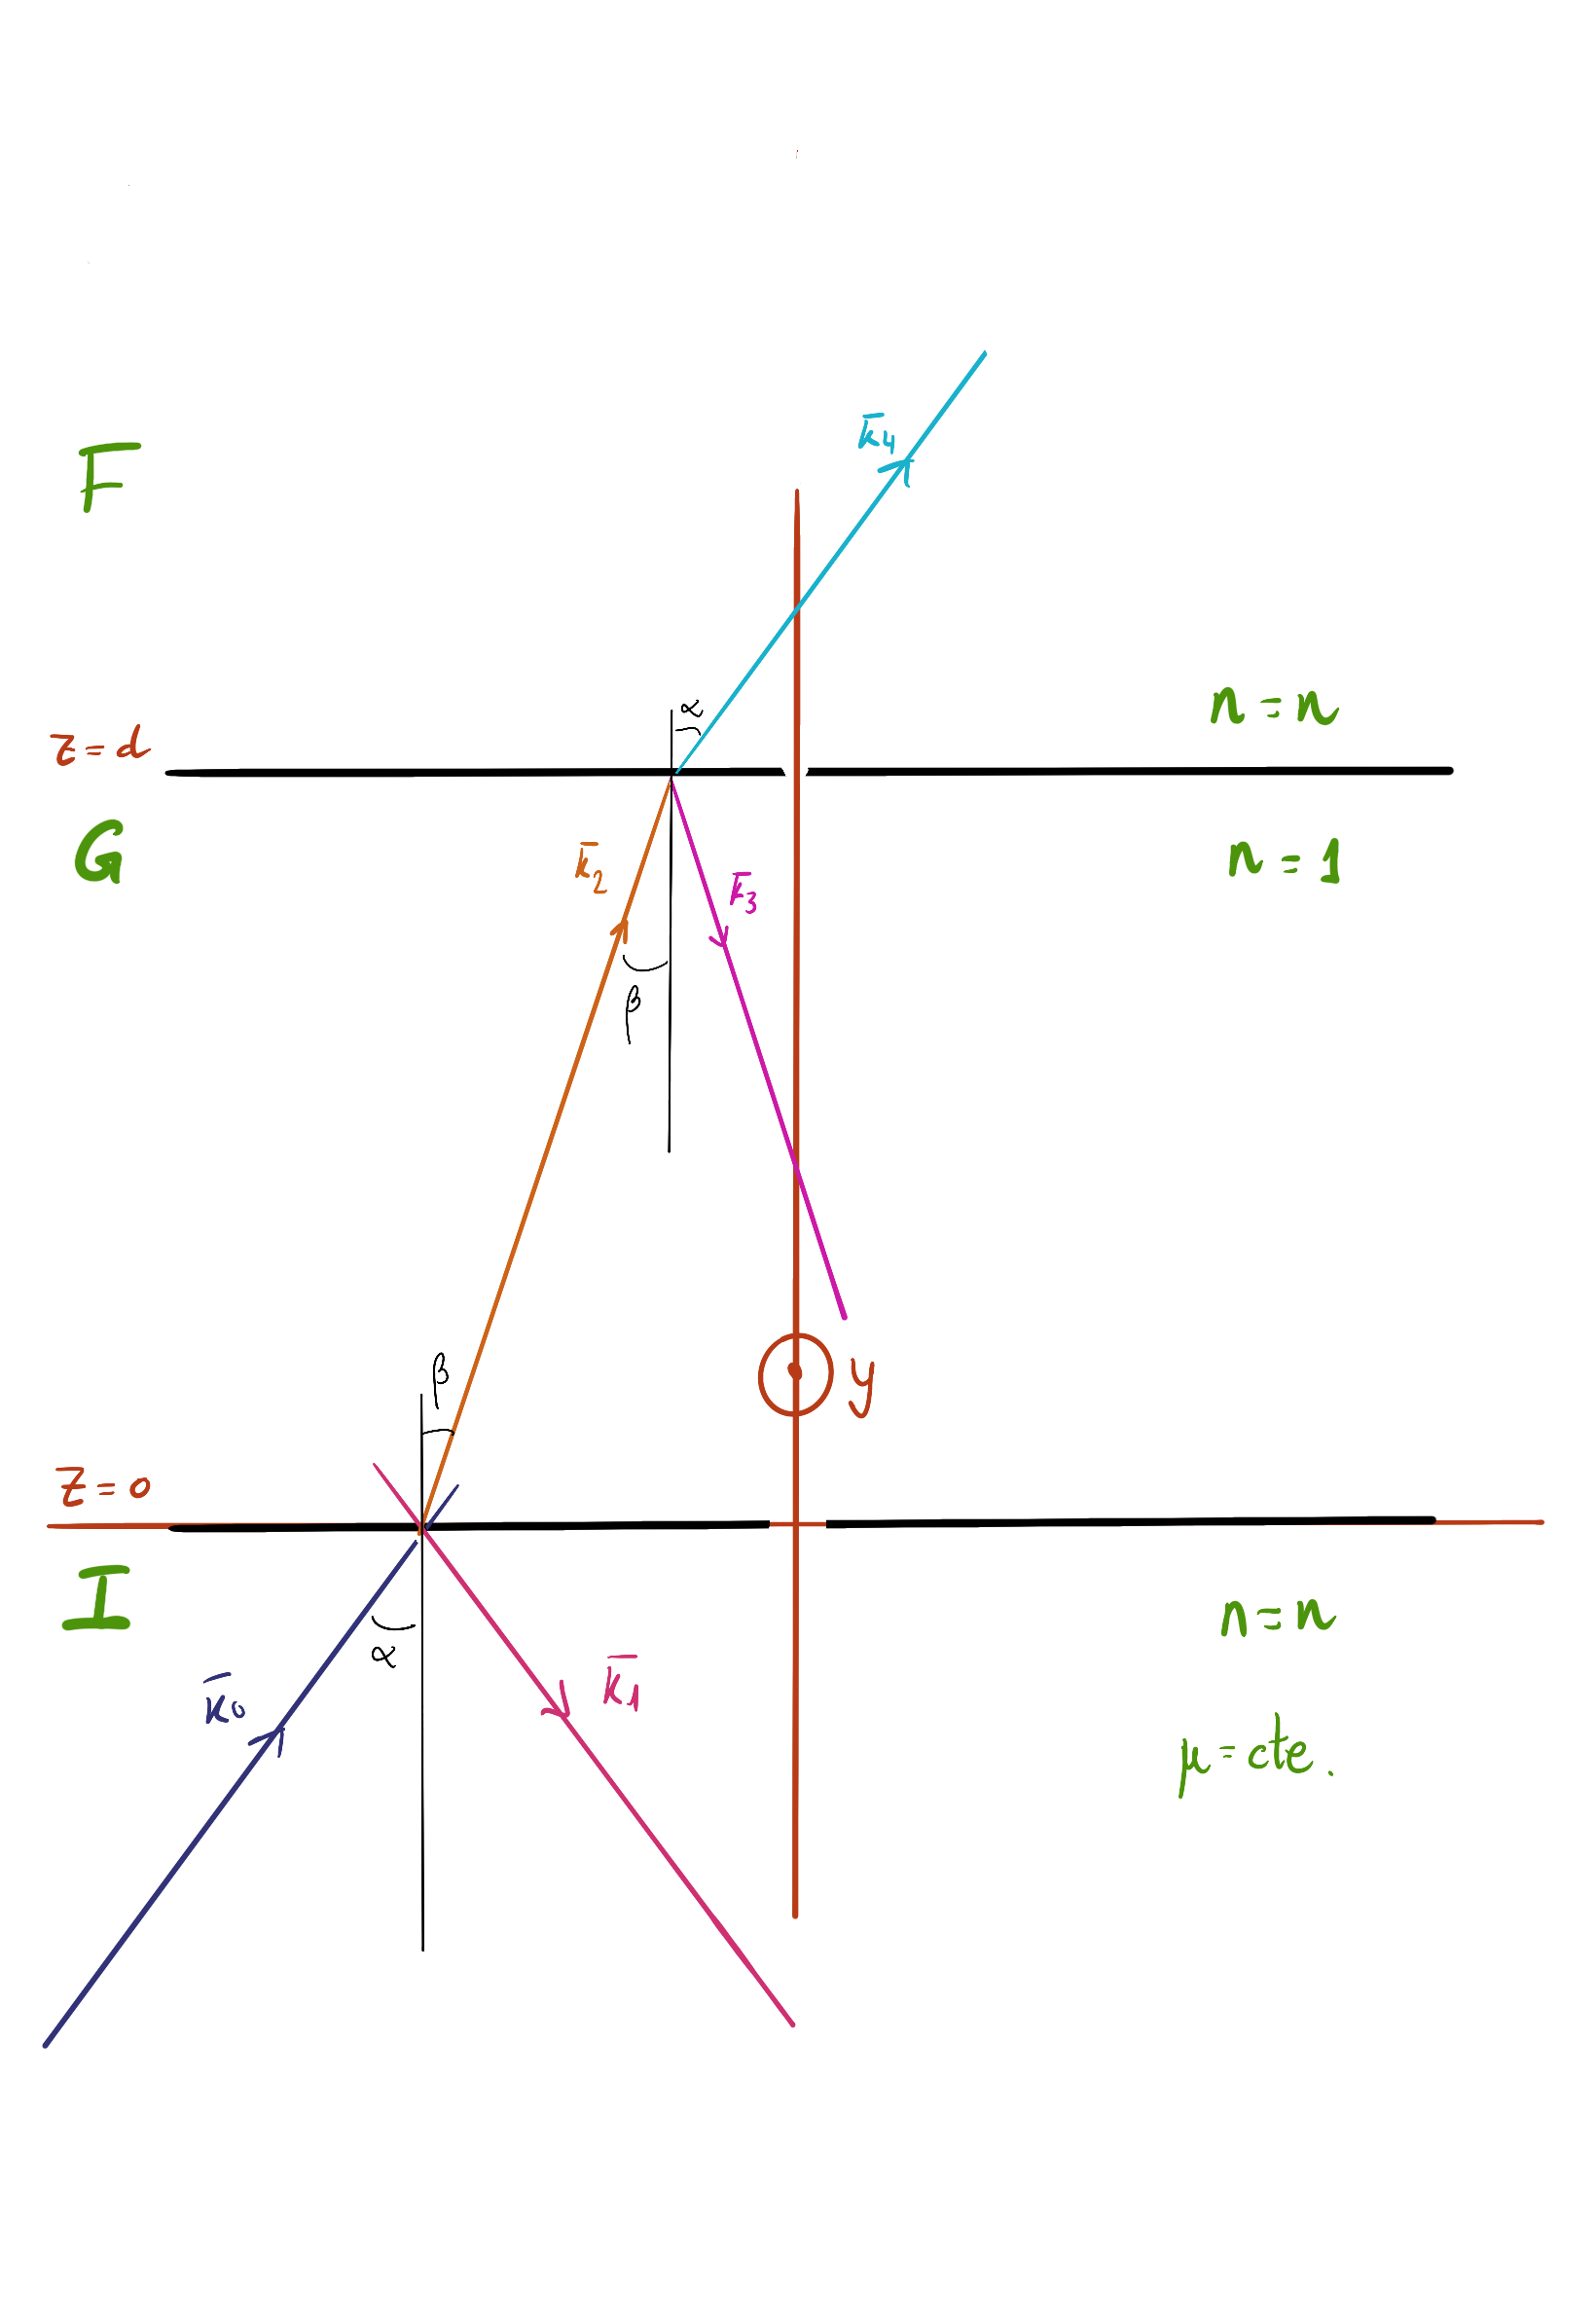
\includegraphics[width=7cm]{figures/Sandwich.png}
	\centering
	\caption{A plane wave trapped between two interphase.}
\end{figure}

In the gap there is also a forward-going wave (the sum of all forward-reflected waves) and a backward-going wave (the sum of all backward-reflected waves). In the transmitted slab there is only a forward-going wave (the sum of all transmitted waves). Note that all materials are lossless so that $n$ and $k$ are real-valued. The waves are all assumed to have linear polarization:

\begin{equation}
	\begin{split}
		&\mathbf{E}_{I}=\hat{\boldsymbol{\epsilon}}_{0} E_{0} e^{i\left(\frac{n}{c} \omega_{0} \hat{\mathbf{k}} \cdot \mathbf{x}-\omega_{0} t\right)}+\hat{\boldsymbol{\epsilon}}_{1} E_{1} e^{i\left(\frac{n}{c} \omega_{\mathbf{1}} \hat{\mathbf{k}}_{1} \cdot \mathbf{x}-\omega_{1} t\right)}, \\
		&\mathbf{E}_{G}=\hat{\boldsymbol{\epsilon}}_{2} E_{2} e^{i\left(\frac{1}{c} \omega_{2} \hat{\mathbf{k}}_{2} \cdot \mathbf{x}-\omega_{2} t\right)}+\hat{\boldsymbol{\epsilon}}_{3} E_{3} e^{i\left(\frac{1}{c} \omega_{3} \hat{\mathbf{k}}_{3} \cdot \mathbf{x}-\omega_{3} t\right)}, \\
		&\mathbf{E}_{F}=\hat{\boldsymbol{\epsilon}}_{4} E_{4} e^{i\left(\frac{n}{c} \omega_{4} \hat{\hat{k}}_{4} \cdot(\mathbf{x}-\mathbf{d})-\omega_{4} t\right)}.
	\end{split}
\end{equation}

What are spatial boundary conditions? The boundary conditions must hold for all time and all points on the boundary. This means that the exponentials must match at $z=0$ and $z=d$, leading to:

\begin{equation}
	\begin{split}
		&{\left[e^{i\left(\frac{n}{c} \omega_{0} \hat{\mathbf{k}} \cdot \mathbf{x}-\omega_{0} t\right)}=e^{i\left(\frac{n}{c} \omega_{1} \hat{\mathbf{k}}_{\mathbf{i}} \cdot \mathbf{x}-\omega_{1} t\right)}=e^{i\left(\frac{1}{c} \omega_{2} \hat{\mathbf{k}}_{2} \cdot \mathbf{x}-\omega_{2} t\right)}=e^{i\left(\frac{1}{c} \omega_{3} \hat{\mathbf{k}}_{\mathbf{3}} \cdot \mathbf{x}-\omega_{3} t\right)}\right]_{z=0},} \\
		&{\left[e^{i\left(\frac{1}{c} \omega_{2} \left.\hat{\mathbf{k}}_{2} \cdot \mathbf{x}-\omega_{2} t\right)\right.}=e^{i\left(\frac{1}{c} \omega_{3} \hat{\mathbf{k}}_{3} \cdot \mathbf{x}-\omega_{3} t\right)}=e^{i\left(\frac{n}{c} \omega_{4} \hat{\mathbf{k}}_{4} \cdot(\mathbf{x}-\mathbf{d})-\omega_{4} t\right)}\right]_{z=d}}
	\end{split}
\end{equation}

These two sets of equations must be true for all times $t$, so that the coefficients of $t$ must match independently, leading to $\omega_{0}=\omega_{1}=\omega_{2}=\omega_{3}=\omega_{4}=\omega$. With the time components all cancelled out, we can simplify to something more handleable as:

\begin{equation}
	\left[n \hat{\mathbf{k}} \cdot \mathbf{x}=n \hat{\mathbf{k}}_{1} \cdot \mathbf{x}=\hat{\mathbf{k}}_{\mathbf{2}} \cdot \mathbf{x}=\hat{\mathbf{k}}_{3} \cdot \mathbf{x}\right]_{z=0} \text { and }\left[\hat{\mathbf{k}}_{\mathbf{2}} \cdot \mathbf{x}=\hat{\mathbf{k}}_{3} \cdot \mathbf{x}=n \hat{\mathbf{k}}_{4} \cdot(\mathbf{x}-\mathbf{d})\right]_{z=d}
\end{equation}

All the wave vectors lie in the same plane. We can assume we have aligned the plane of incidence with the $x-z$ plane. As a result, none of the wave vectors have any $y$ components. Expand the vectors into $x$ and $z$ components and define these components in terms of the angles from the $z$ axis (for example $\left.k_{x}=k \sin \theta_{i}, k_{z}=k \cos \theta_{i}\right) .$ Evaluate at $z=0$ and $z=d$. Note that evaluating at specific $z$ locations reduces the $z$-component equations down to just a bunch of constants. They have no meaning at this point because we can always suck a constant phase factor into the remaining undetermined coefficients $E_{0}, E_{1}$, etc. Because of the lack of meaningful information, we completely drop the $z$ components. All that remains is the $x$ components, which allow us to identify the angles as:

\begin{equation}
	\theta_{I}=\theta_{R}, \quad \theta_{G, I}=\theta_{G, R}, \quad \theta_{I}=\theta_{F, I},\quad  n \sin \theta_{I}=\sin \theta_{G, I}, \quad \sin \theta_{G, I}=n \sin \theta_{F, I}.
\end{equation}

Congratulations to us! We have just derived Snell's law. This will allow us to express all relations in terms of the incident angle. Note that because we are dealing with plane waves and flat interfaces, we can work with all these fields at the lateral position
$x = 0$ without any loss of generality. In addition, we can evaluate the fields at time $t = 0$ without any loss of generality. Lastly, we use the shorthand notation $\cos \theta_{g,i} = \sqrt{1 - n^{2} \sin^{2} \theta_{i}}$ . With these simplifications, the fields become:

\begin{equation}
	\begin{split}
		\begin{aligned}
			&\mathbf{E}_{I}=\hat{\mathbf{\epsilon}}_{0} E_{0} e^{i \frac{n}{c} \omega \cos \theta_{i} z}+\hat{\boldsymbol{\epsilon}}_{1} E_{1} e^{-i \frac{n}{c} \omega \cos \theta_{i} z}, \\
			&\mathbf{E}_{G}=\hat{\boldsymbol{\epsilon}}_{2} E_{2} e^{i \frac{1}{c} \omega \cos \theta_{g, i} z}+\hat{\boldsymbol{\epsilon}}_{3} E_{3} e^{-i \frac{1}{c} \omega \cos \theta_{g, i} z}, \\
			&\mathbf{E}_{F}=\hat{\mathbf{\epsilon}}_{4} E_{4} e^{i \frac{n}{c} \omega \cos \theta_{i}(z-d)}.
		\end{aligned}
	\end{split}
\end{equation}

This is going to be our starting point for the present waves in our system. We have two possible cases: The polarisation of the wave being $\perp$ to the plane of incidence and polarisation contained in the plane. Let's study both cases:

\subsubsection*{Perpendicular}

This means that we leave the polarisation to fall in the $y-$direction. The electric and magnetic fields ($\mathbf{B} = \tfrac{n}{c} \hat{\mathbf{k}} \times \mathbf{E}$) are:

\begin{equation}
	\begin{split}
		&\mathbf{E}_{I}=\hat{\mathbf{y}} E_{0} e^{i \frac{n}{c} \omega \cos \theta_{i} z}+\hat{\mathbf{y}} E_{1} e^{-i \frac{n}{c} \omega \cos \theta_{i} z},\\
		&\mathbf{E}_{G}=\hat{\mathbf{y}} E_{2} e^{i \frac{1}{c} \omega \cos \theta_{g, i} z}+\hat{\mathbf{y}} E_{3} e^{-i \frac{1}{c} \omega \cos \theta_{g, i} z},\\
		&\mathbf{E}_{F}=\hat{\mathbf{y}} E_{4} e^{i \frac{n}{c} \omega \cos \theta_{i}(z-d)},\\
		&\mathbf{B}_{I}=\tfrac{n}{c}\left(\sin \theta_{i} \hat{\mathbf{z}}-\cos \theta_{i} \hat{\mathbf{x}}\right) E_{0} e^{i \frac{n}{c} \omega \cos \theta_{i} z}+\tfrac{n}{c}\left(\sin \theta_{i} \hat{\mathbf{z}}+\cos \theta_{i} \hat{\mathbf{x}}\right) E_{1} e^{-i \frac{n}{c} \omega \cos \theta_{i} z,}\\
		&\mathbf{B}_{G}=\tfrac{1}{c}\left(n \sin \theta_{i} \hat{\mathbf{z}}-\cos \theta_{g, i} \hat{\mathbf{x}}\right) E_{2} e^{i \frac{1}{c} \omega \cos \theta_{g, i} z}+\tfrac{1}{c}\left(n \sin \theta_{i} \hat{\mathbf{z}}+\cos \theta_{g, i} \hat{\mathbf{x}}\right) E_{3} e^{-i \frac{1}{c} \omega \cos \theta_{g, i} z},\\
		&\mathbf{B}_{F}=\tfrac{n}{c}\left(\sin \theta_{i} \mathbf{z}-\cos \theta_{i} \mathbf{x}\right) E_{4} e^{i \tfrac{n}{c} \omega \cos \theta_{i}(z-d)}.
	\end{split}
\end{equation}

Which will have to follow the boundary conditions\footnote{As we are dealing with dielectric materials, we must apply all boundary conditions.} when no charges or currents are present:

\begin{equation}
	\begin{split}
	\left[\epsilon_{2} \mathbf{E}_{2} \cdot \mathbf{n}=\epsilon_{1} \mathbf{E}_{1} \cdot \mathbf{n}\right]_{z=0,d} \quad&, \quad\left[\mathbf{E}_{2} \times \mathbf{n}=\mathbf{E}_{1} \times \mathbf{n}\right]_{z=0,d},\\
	\left[\mathbf{B}_{2} \cdot \mathbf{n}=\mathbf{B}_{1} \cdot \mathbf{n}\right]_{z=0,d} \quad&, \quad\left[\tfrac{1}{\mu_{2}} \mathbf{B}_{2} \times \mathbf{n}=\tfrac{1}{\mu_{1}} \mathbf{B}_{1} \times \mathbf{n}\right]_{z=0,d}.
	\end{split}
\end{equation}

So 8 boundary conditions in total. With good manners, patience and a beverage by your side, one can arrive to the following relations;

\begin{equation}\label{interfaseconditions}
	\begin{split}
		&0=0 \quad (\text{2 equations will give this requirement}),\\
		&E_{2}+E_{3}=E_{0}+E_{1} \quad (\text{2 equations will give this requirement}),\\
		&E_{2}-E_{3}=b\left(E_{0}-E_{1}\right),\\
		&E_{4}=E_{2} e^{i a}+E_{3} e^{-i a} \quad (\text{2 equations will give this requirement}),\\
		&b E_{4}=E_{2} e^{i a}-E_{3} e^{-i a}.
	\end{split}
\end{equation}

where $b=\frac{n \cos \theta_{i}}{\sqrt{1-n^{2} \sin ^{2} \theta_{i}}}$ and  $a=\frac{1}{c} \omega d \sqrt{1-n^{2} \sin ^{2} \theta_{i}}$.

Considering that the incident strength $E_{0}$ is taken to be a known, we have four independent equations above in four unknowns and can therefore solve uniquely for the different field strengths. After much algebra (mathematica in my case), we solve this system of equations as:

\begin{equation}
	\begin{split}
		&\frac{E_{1}}{E_{0}}=\frac{\left(1-b^{2}\right) i \sin a}{2 b \cos a-\left(1+b^{2}\right) i \sin a},\\
		&\frac{E_{2}}{E_{0}}=\frac{b(1+b)(\cos a-i \sin a)}{2 b \cos a-i\left(1+b^{2}\right) \sin a},\\
		&\frac{E_{3}}{E_{0}}=\frac{b(1-b)(\cos a+i \sin a)}{2 b \cos a-i\left(1+b^{2}\right) \sin a},\\
		&\frac{E_{4}}{E_{0}}=\frac{2 b}{2 b \cos a-i\left(1+b^{2}\right) \sin a}.\\
	\end{split}
\end{equation}

We now want to find the fraction of reflected and transmitted power by taking the magnitude squared of the first and last equation. We have to be careful because beyond the critical angle of total internal reflection, $a$ and $b$ become purely imaginary, but we can still have valid transmission via the evanescent modes. Let us approach the two cases separately. Below the critical angle, $a$ and $b$ are purely real-valued, leading to:

\begin{equation}
	R=\left|\frac{E_{1}}{E_{0}}\right|^{2}=\frac{\left(1-b^{2}\right)^{2} \sin ^{2} a}{4 b^{2} \cos ^{2} a+\left(1+b^{2}\right)^{2} \sin ^{2} a}.
\end{equation}

And the transmitted power is:

\begin{equation}
	T=\left|\frac{E_{4}}{E_{0}}\right|^{2}=\frac{4 b^{2}}{4 b^{2} \cos ^{2} a+\left(1+b^{2}\right)^{2} \sin ^{2} a}.
\end{equation}

As for the case we want to go beyond the critical angle of internal reflection, we have to notice than $a,b$ become imaginary. We can rephrase them, for convenience, as $a = i \alpha$ and $b= - i \beta$ so the reflected and transmitted powers in this case become:

\begin{equation}
	\begin{split}
			&R=\left|\frac{E_{1}}{E_{0}}\right|^{2}=\frac{\left(1+\beta^{2}\right)^{2} \sinh ^{2}(\alpha)}{4 \beta^{2} \cosh ^{2}(\alpha)+\left(1-\beta^{2}\right)^{2} \sinh ^{2}(\alpha)},\\
			&T=\left|\frac{E_{4}}{E_{0}}\right|^{2}=\frac{4 \beta^{2}}{4 \beta^{2} \cosh ^{2}(\alpha)+\left(1-\beta^{2}\right)^{2} \sinh ^{2}(\alpha)}.
	\end{split}
\end{equation}

\subsubsection*{Contained}

We just have to do again  the same thing for the polarization where the electric fields are in the plane of incidence. All of the forward going waves have $\mathbf{E}$ fields pointing in the negative- $x /$ positive- $z$ direction and all the backwards going waves have $\mathbf{E}$ pointing in the positive- $x /$ positive- $z$ direction. Using $\mathbf{B}=(n / c) \hat{\mathbf{k}} \times \mathbf{E}$, we find the fields for parallel polarization are:

\begin{equation}
	\begin{split}
		&\mathbf{E}_{I}=\left(-\cos \theta_{i} \hat{\mathbf{x}}+\sin \theta_{i} \hat{\mathbf{z}}\right) E_{0} e^{i \frac{n}{c} \omega \cos \theta_{i} z}+\left(\cos \theta_{i} \hat{\mathbf{x}}+\sin \theta_{i} \hat{\mathbf{z}}\right) E_{1} e^{-i \frac{n}{c} \omega \cos \theta_{i} z},\\
		&\mathbf{E}_{G}=\left(-\cos \theta_{g, i} \hat{\mathbf{x}}+n \sin \theta_{i} \hat{\mathbf{z}}\right) E_{2} e^{i \frac{1}{c} \omega \cos \theta_{g, i} z}+\left(\cos \theta_{g, i} \hat{\mathbf{x}}+n \sin \theta_{i} \hat{\mathbf{z}}\right) E_{3} e^{-i \frac{1}{c} \omega \cos \theta_{g, i} z},\\
		&\mathbf{E}_{F}=\left(-\cos \theta_{i} \hat{\mathbf{x}}+\sin \theta_{i} \hat{\mathbf{z}}\right) E_{4} e^{i \frac{n}{c} \omega \cos \theta_{i}(z-d)},\\
		&\mathbf{B}_{I}=-\hat{\mathbf{y}}(n / c)\left(E_{0} e^{i \frac{n}{c} \omega \cos \theta_{i} z}+E_{1} e^{-i \frac{n}{c} \omega \cos \theta_{i} z}\right),\\
		&\mathbf{B}_{G}=-\hat{\mathbf{y}}(1 / c)\left(E_{2} e^{i \frac{1}{c} \omega \cos \theta_{g, i} z}+E_{3} e^{-i \frac{1}{c} \omega \cos \theta_{g, i} z}\right),\\
		&\mathbf{B}_{F}=-\hat{\mathbf{y}}(n / c) E_{4} e^{i \frac{n}{c} \omega \cos \theta_{i}(z-d)}.
	\end{split}
\end{equation}

Where, again, $\cos \theta_{g, i}=\sqrt{1-n^{2} \sin ^{2} \theta_{i}}.$ Imposing again eq(\ref{interfaseconditions}), we will arrive to some relations of the amplitude of $\mathbf{E}$ and $\mathbf{B}$. If one solves the system of four equations, the result is:

\begin{equation}
	\begin{split}
		\begin{aligned}
			&\frac{E_{1}}{E_{0}}=\frac{\left(n^{4}-b^{2}\right) i \sin a}{2 n^{2} b \cos a-i\left(n^{4}+b^{2}\right) \sin a}, \\
			&\frac{E_{2}}{E_{0}}=\frac{b n\left(n^{2}+b\right)(\cos a-i \sin a)}{2 n^{2} b \cos a-i\left(n^{4}+b^{2}\right) \sin a},\\
			&\frac{E_{3}}{E_{0}}=\frac{b n\left(n^{2}-b\right)(\cos a+i \sin a)}{2 n^{2} b \cos a-i\left(n^{4}+b^{2}\right) \sin a},\\
			&\frac{E_{4}}{E_{0}}=\frac{2 n^{2} b}{2 n^{2} b \cos a-i\left(n^{4}+b^{2}\right) \sin a}.
		\end{aligned}
	\end{split}
\end{equation}

Which again, being careful about the critical angle, we find below this:

\begin{equation}
	\begin{split}
		&R=\left|\frac{E_{1}}{E_{0}}\right|^{2}=\frac{\left(n^{4}-b^{2}\right)^{2} \sin ^{2} a}{4 n^{4} b^{2} \cos ^{2} a+\left(n^{4}+b^{2}\right)^{2} \sin ^{2} a}, \\
		&T=\left|\frac{E_{4}}{E_{0}}\right|^{2}=\frac{4 n^{4} b^{2}}{4 n^{4} b^{2} \cos ^{2} a+\left(n^{4}+b^{2}\right)^{2} \sin ^{2} a}.
	\end{split}
\end{equation}

With $a,b$ as in the stated in the previous part of the exercise.

\subsubsection{Faraday Rotation During Propagation}\label{Faraday Rotation During Propagation}

Let $k_{L}=\omega n_{L} / c$ and $k_{R}=\omega n_{R} / c .$ Left and right circularly polarized plane waves with the same amplitude and frequency propagating along the $z$ -axis in the medium we want to study. Then the plane waves should look like:

\begin{equation}
	\mathbf{E}_{L}(z, t)=E(\hat{\mathbf{x}}+i \hat{\mathbf{y}}) \exp \left[i\left(k_{L} z-\omega t\right)\right], \quad \mathbf{E}_{R}(z, t)=E(\hat{\mathbf{x}}-i \hat{\mathbf{y}}) \exp \left[i\left(k_{R} z-\omega t\right)\right].
\end{equation}

In this basis, the given electric field is given by:

\begin{equation}
	\mathbf{E}(z=0, t)=\frac{1}{2}\left[\mathbf{E}_{L}(z=0, t)+\mathbf{E}_{R}(z=0, t)\right].
\end{equation}

Therefore, at other points in space we find:

\begin{equation}
	\begin{split}
		\mathbf{E}(z, t) &=\frac{1}{2}\left[\mathbf{E}_{L}(z, t)+\mathbf{E}_{R}(z, t)\right], \\
		&=\frac{1}{2} E\left[e^{i k_{L} z}+e^{i k_{R} z}\right] e^{-i \omega t} \hat{\mathbf{x}}+\frac{i}{2} E\left[e^{i k_{L} z}-e^{i k_{R} z}\right] e^{-i \omega t} \hat{\mathbf{y}}.
	\end{split}
\end{equation}

The field will be linearly polarized along $\hat{\mathbf{y}}$ when:

\begin{equation}
	e^{i k_{L} z}=-e^{i k_{R} z}=e^{i k_{R} z} e^{\pm i m \pi}, \quad m=1,3,5, \ldots
\end{equation}

And this only happens when $z$ takes values of the form:
\begin{equation}
	z=\pm \frac{m \pi}{k_{L}-k_{R}}=\pm \frac{m \pi c / \omega}{n_{L}-n_{R}}, \quad m=1,3,5, \ldots
\end{equation}

\subsubsection{Charged Particle Motion in a Circular Polarized wave}\label{Charged Particle Motion in a Circular Polarized wave}


\textbf{a):}

The physical electric field is:

\begin{equation}
	\mathrm{E}(z, t)=(\hat{\mathbf{x}}+i \hat{\mathbf{y}}) E_{0} e^{+i(k z-\omega t)}+(\hat{\mathbf{x}}-i \hat{\mathbf{y}}) E_{0} e^{-i(k z-\omega t)}.
\end{equation}

And the corresponding magnetic field can be obtained from:

\begin{equation}
	\mathrm{B}(z, t)=\frac{1}{c} \hat{\mathbf{z}} \times \mathrm{E}(z, t).
\end{equation}

Therefore (Long computation):

\begin{equation}
	\begin{split}
		\frac{d \mathbf{v}}{d t} &=\frac{q}{m}\left[\mathbf{E}+\mathbf{v} \times \frac{1}{c}(\hat{\mathbf{z}} \times \mathbf{E})\right]= \\
		&=\frac{q}{m}\left[\left(1-\frac{v_{z}}{c}\right) \mathbf{E}+\hat{\mathbf{z}} \frac{\mathbf{v} \cdot \mathbf{E}}{c}\right] =\\
		&=\frac{q}{m}\left(1-\frac{v_{z}}{c}\right) E_{0}\left\{(\hat{\mathbf{x}}+i \hat{\mathbf{y}}) E_{0} e^{+i(k z-\omega t)}+(\hat{\mathbf{x}}-i \hat{\mathbf{y}}) E_{0} e^{-i(k z-\omega t)}\right\} +\\
		&\quad +\hat{\mathbf{z}} \frac{q E_{0}}{m c}\left\{\left(v_{x}+i v_{y}\right) e^{+i(k z-\omega t)}+\left(v_{x}-i v_{y}\right) e^{-i(k z-\omega t)}\right\}.
	\end{split}
\end{equation}

So the required velocities are:

\begin{equation}\label{velocities}
	\begin{split}
		\frac{d v_{z}}{d t}&=\frac{1}{2} \Omega\left\{v_{+} e^{+i(k z-\omega t)}+v_{-} e^{-i(k z-\omega t)}\right\}, \\
		\frac{d v_{\pm}}{d t}&=\Omega\left(c-v_{z}\right) e^{\mp i(k z-\omega t)},
	\end{split}
\end{equation}

Where $v_{\pm}=v_{x} \pm i v_{y}$ and $\Omega=2 q E_{0} / m c$.

\textbf{b):}

Now define $\ell_{\pm}=v_{\pm} e^{\pm i(k z-\omega t)} \pm i c \Omega / \omega$ so

\begin{equation}\label{vzvelocity}
	\frac{d v_{z}}{d t}=\frac{1}{2} \Omega\left(\ell_{+}+\ell_{-}\right)
\end{equation}

On the other hand,

\begin{equation}
	\frac{d \ell_{\pm}}{d t}=\frac{d v_{\pm}}{d t} e^{\pm i(k z-\omega t)} \mp i \omega v_{\pm} e^{\pm i(k z-\omega t)}=\Omega\left(c-v_{z}\right) \mp i \omega v_{\pm} e^{\pm i(k z-\omega t)}.
\end{equation}
	
Therefore, using (\ref{velocities}),

\begin{equation}
	\frac{d}{d t}\left(\ell_{-}-\ell_{+}\right)=-i \omega\left[v_{+} e^{i(k z-\omega t)}+v_{-} e^{-i(k z-\omega t)}\right]=-\frac{2 i \omega}{\Omega} \frac{d v_{z}}{d t}.
\end{equation}

So we can conclude that:

\begin{equation}
	\frac{d}{d t}\left\{v_{z}-i \frac{\Omega}{2 \omega}\left(l_{+}-\ell_{-}\right)\right\}=0
\end{equation}

Hence, a constant of the motion is:

\begin{equation}
	K=v_{z}(0)-i \frac{\Omega}{2 \omega}\left[l_{+}(0)-\ell_{-}(0)\right] .
\end{equation}

\textbf{c):}

Differentiating (\ref{vzvelocity}) gives:

\begin{equation}
	\frac{d^{2} v_{z}}{d t^{2}}=\frac{\Omega}{2}\left[\frac{d \ell_{+}}{d t}+\frac{d \ell_{-}}{d t}\right]=\Omega^{2}\left(c-v_{z}\right)-\frac{1}{2} i \omega \Omega\left\{v_{+} e^{i(k z-\omega t)}-v_{-} e^{-i(k z-\omega t)}\right\} .
\end{equation}

But, recall that $\ell_{+}-\ell_{-}=v_{+} e^{i(k z-\omega t)}-v_{-} e^{-i(k z-\omega t)}+2 i \Omega c / \omega$ so
	
\begin{equation}
	\frac{d^{2} v_{z}}{d t^{2}}=\Omega^{2}\left(c-v_{z}\right)-\frac{1}{2} i \omega \Omega\left\{\ell_{+}-\ell_{-}-2 i \Omega c / \omega\right\}=-\left(\Omega^{2}+\omega^{2}\right) v_{z}+\omega^{2} K.
\end{equation}

Now, imposing some initial conditions as $v(0)=0$ and $\ell_{\pm}(0)=\pm i c \Omega / \omega$, in which case, $\omega^{2} K=c \Omega^{2} .$ Hence, if we define:
	
\begin{equation}
	P=c \Omega^{2} \quad \text { and } \quad \Omega_{0}^{2}=\Omega^{2}+\omega^{2}
\end{equation}

The EOM for $v_{z}$ is
	
\begin{equation}
	\frac{d^{2} v_{z}}{d t^{2}}+\Omega_{0}^{2} v_{z}=P.
\end{equation}

This is solved by writing
	
\begin{equation}
	\frac{d^{2}}{dt^{2}}\left(v_{z}-\frac{P}{\Omega_{0}^{2}}\right)+\Omega_{0}^{2}\left(v_{z}-\frac{P}{\Omega_{0}^{2}}\right)=0.
\end{equation}

so $v_{z}(t)=A \sin \Omega_{0} t+B \cos \Omega_{0} t+P / \Omega_{0}^{2} .$ The initial conditions $v_{z}(0)=\dot{v}_{z}(0)=0$ determine the constants and we finally can get:
	
\begin{equation}
	\begin{split}
		v_{z}(t)=\frac{P}{\Omega_{0}^{2}}\left(1-\cos \Omega_{0} t\right), \\
		a_{z}(t)=\frac{P}{\Omega_{0}^{2}} \sin \Omega_{0} t.
	\end{split}
\end{equation}

No steady acceleration occurs; the particle cyclically accelerates and decelerates as it propagates along the $z$ -axis.

\subsubsection{E: A Wave and Some Boundary Conditions}\label{E: A Wave and Some Boundary Conditions}

\textbf{1):}

The first thing we should do, as always, is to draw a sketch of the geometrical set-up is described in the statement of the problem. It roughly looks like:
	
\begin{figure}[h!]
	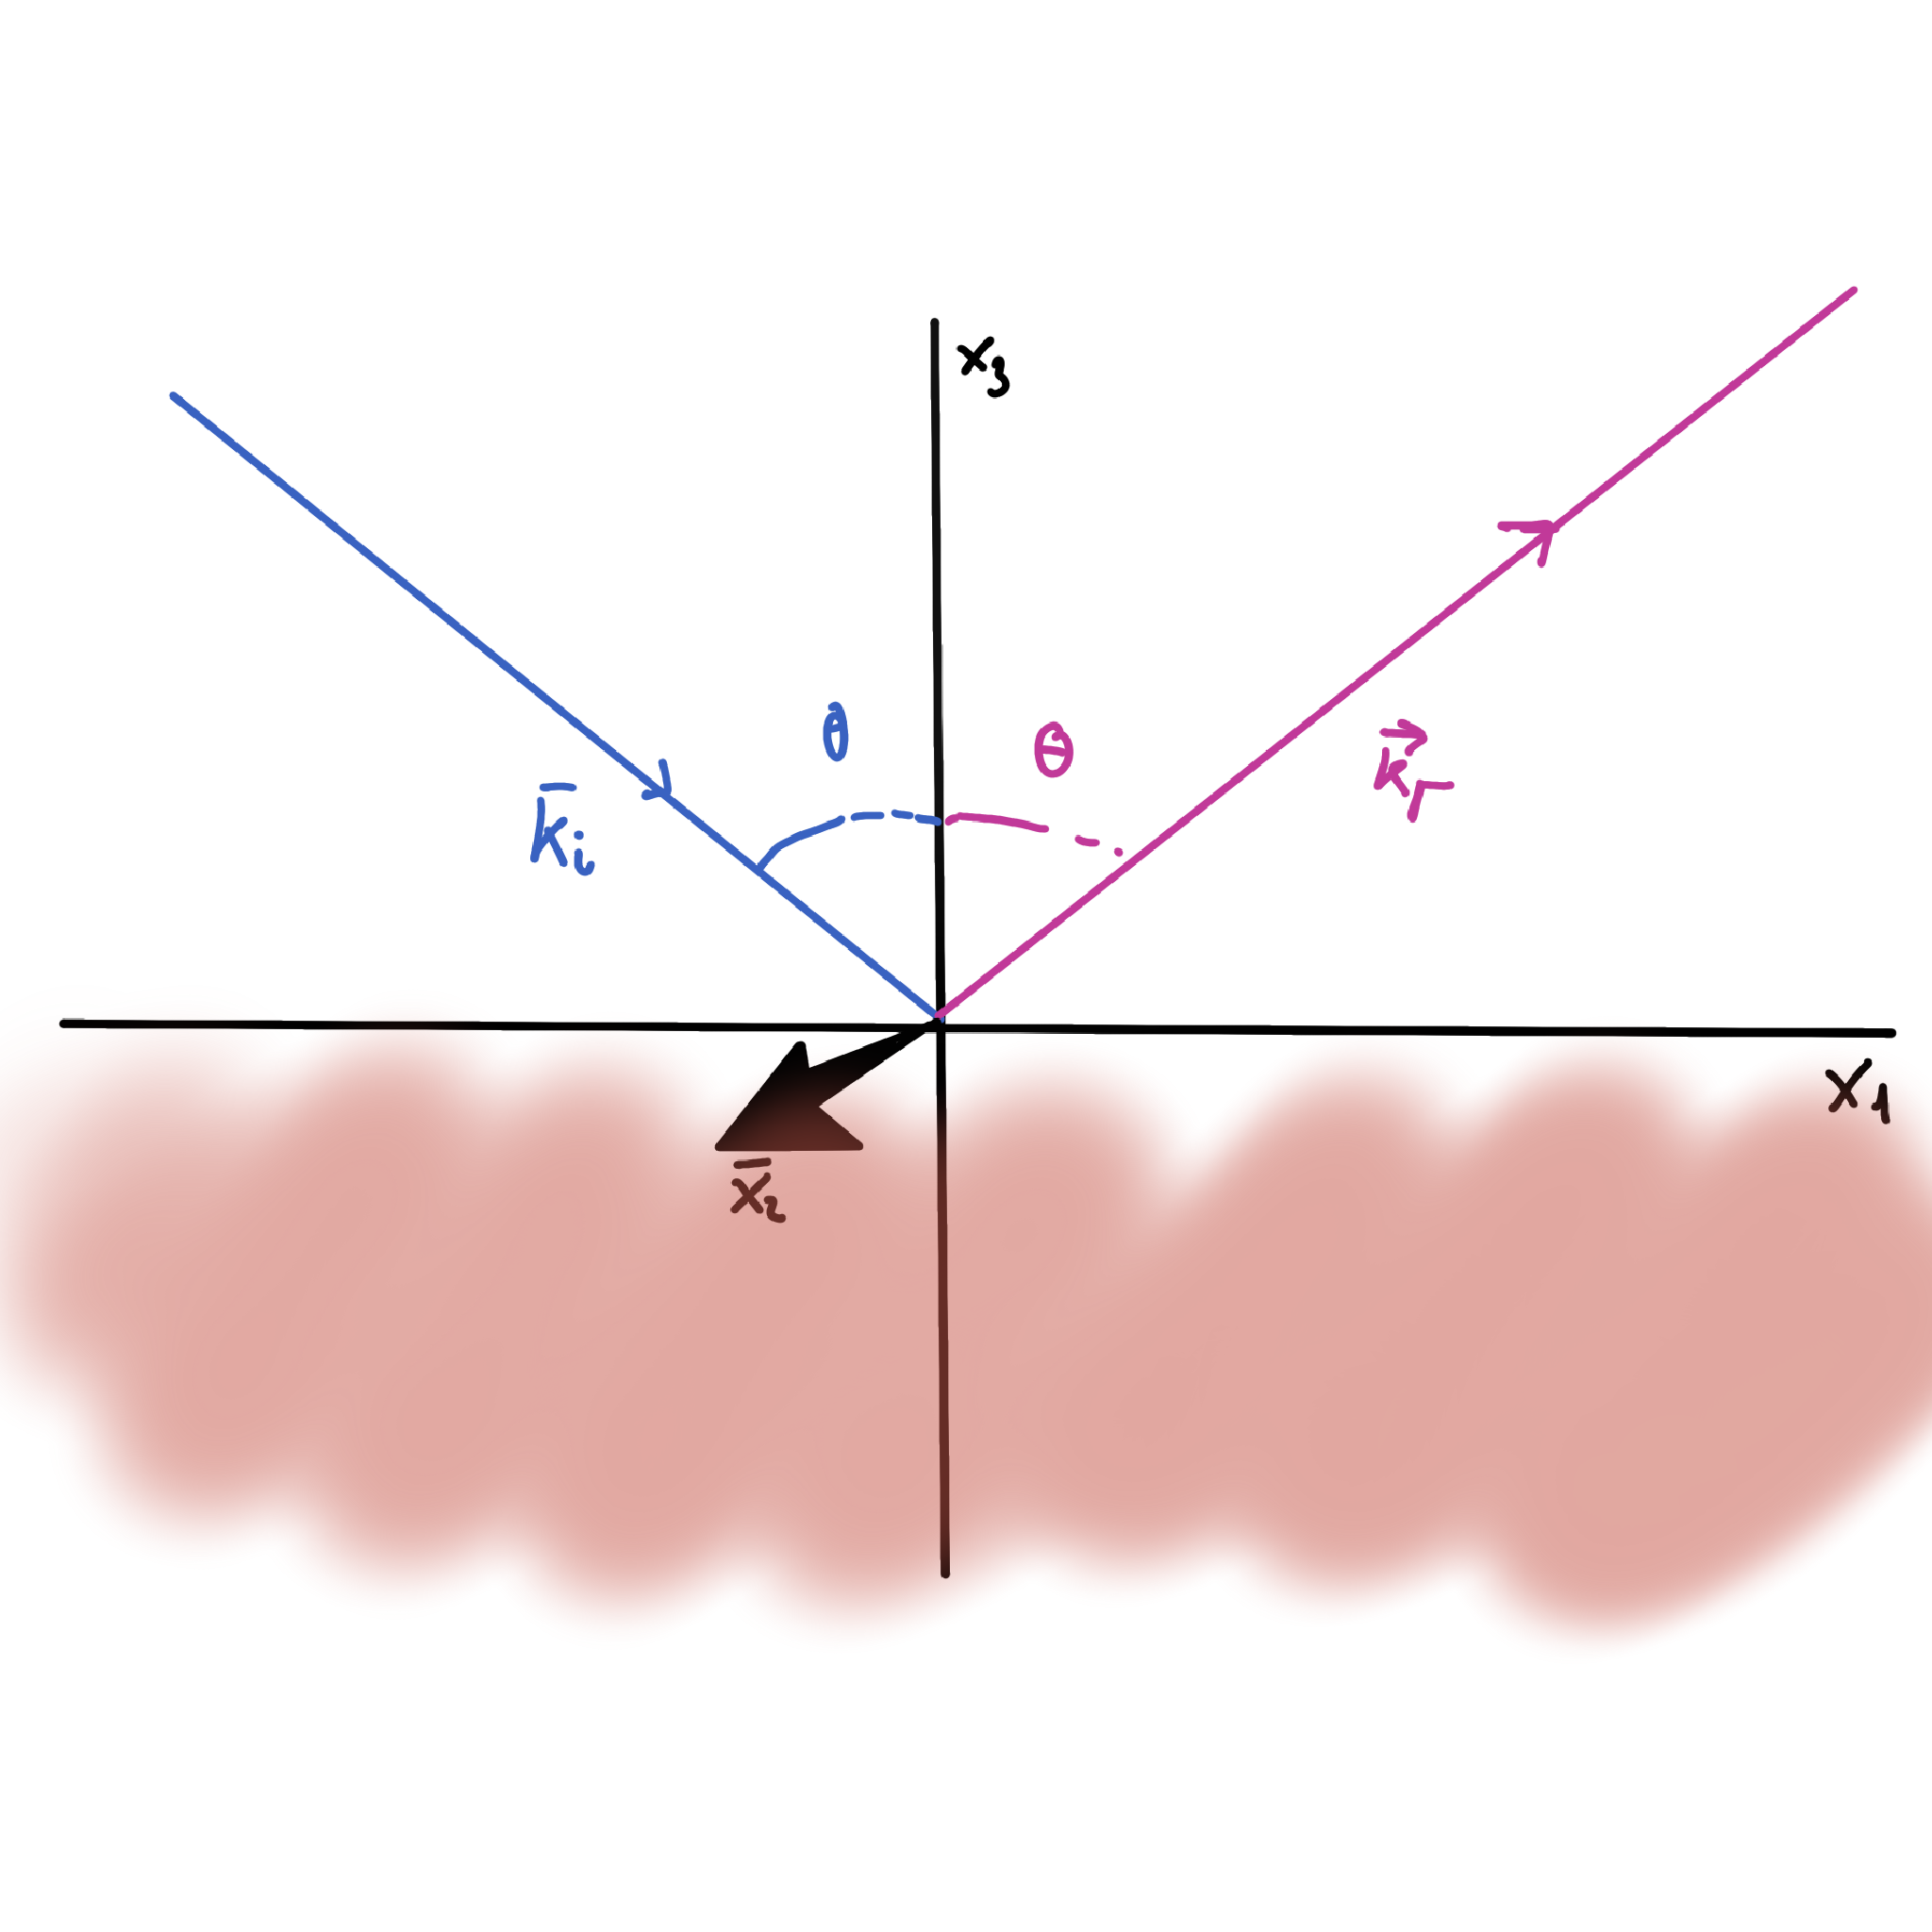
\includegraphics[width=6cm]{figures/X3plane.png}
	\centering
	\caption{A sketch of the planes and waves in this problem.}
\end{figure}
	
With fields given by:
\begin{subequations}
	\begin{align}
		\vec{E}_{i}(\vec{x}, t)&=\vec{E}_{0} e^{\mathrm{i} \vec{k} \cdot \vec{x}-\mathrm{i} \omega t} ,\\
		\vec{B}_{i}(\vec{x}, t)&=\frac{\hat{k}}{c} \times \vec{E}_{i},
	\end{align}
\end{subequations}

where $\{i,r\}$ sub-indices stand for incident and reflected waves. Let us now suppose that we have the incident wave on a perfect conductor at $x_{3}=0$. The plane of incidence is fixed by $\hat{k}$ and $\hat{x}_{3}$. As we did in the previous problem \textit{A Sandwich of light}, we will have to consider perpendicular and parallel polarization with respect the plane that the wave vector and $\hat{x}_{3}$ form. Without any loss of generality, the wave vector can be written as:
	
\begin{equation}
	\vec{k} = k_{2} \hat{x}_{2} - k_{3}\hat{x}_{3}.
\end{equation}

We can always rotate the system such that the wave vector is contained in the plane $\hat{x}_{2} - \hat{x}_{3}$. The problem does not state any other type of material in $x_{3} <0$, so we keep the same permeabilities as in $x_{3}>0$ ($\mu_{2} = \mu_{1}$ and $\epsilon_{2} = \epsilon_{1}$).   Now that we have $\vec{k}$ fixed in some plane, let us check the boundary conditions at $x_{3}=0$. That for the wave vector takes the well known form of:
	
\begin{equation}
	\left[\mathbf{k}_{i} \cdot \mathbf{x}=\mathbf{k}_{r} \cdot \mathbf{x}\right]_{x_{3}=0}
\end{equation}

While the boundary condition for the component of fields $\mathbf{E}$ and $\mathbf{B}$ are given at $x_{3} =0$ by:

\begin{equation}\label{eq:boundaryconditionsfields}
	\begin{split}
		\left[\mathbf{E}_{1} \cdot \mathbf{n}= \mathbf{E}_{2} \cdot \mathbf{n}\right]_{x_{3}=0} \quad&, \quad\left[\mathbf{E}_{1} \times \mathbf{n}=\mathbf{E}_{2} \times \mathbf{n}\right]_{x_{3}=0},\\
		\left[\mathbf{B}_{1} \cdot \mathbf{n}=\mathbf{B}_{2} \cdot \mathbf{n}\right]_{x_{3}=0} \quad&, \quad\left[ \mathbf{B}_{1} \times \mathbf{n}= \mathbf{B}_{2} \times \mathbf{n}\right]_{x_{3}=0}.
	\end{split}
\end{equation}
	
These both packages have to be satisfied at any moment in time\footnote{But notice that we are dealing with a conducting material. This means that there should not be any fields $\textbf{inside}$, but there can be fields outside, so $E\cdot n$ does not make sense to set to 0. On top of that, as we have a perfect conducting material, any incident electric field on the surface can induce a current $\vec{j}$, with surface energy density $\sigma$. This can be observed checking the four boundary condition equations from Maxwell. Although to discuss this is not the scope of the problem, it is important to notice it.}. We can notice that, although the norm form both wave vector $\mathbf{k}_{i,r}$ is the same, the $x_{3}$ will change in sign, as the wave is reflected. All in all, the most general expression for $\mathbf{E}$, for this region of space that we can think of, is a linear combination of the incoming wave and the reflected one, as:
	
\begin{equation}
	\mathbf{E}_{1} = \vec{E}_{0i} e^{i\left(k_{2} \hat{x}_{2} - k_{3} \hat{x}_{3} -\omega t\right)} + \vec{E}_{0r} e^{i\left(k_{2} \hat{x}_{2} + k_{3} \hat{x}_{3} -\omega t\right)}
\end{equation}

Observe that we have not specified yet the polarisation of this field. This depends if we want to consider it perpendicular o parallel to the incidence plane. Let's do that now:\\
	
\textbf{PERPENDICULAR}
	
In this case, that means that $\vec{E}_{0i,r} = E_{0i,r} \hat{x}_{1}$.  Then, imposing boundary conditions (\ref{eq:boundaryconditionsfields}) we obtain that:
	
\begin{equation}
	\begin{split}
		\mathbf{E}_{1}& \times \hat{n} = 0 \qquad \rightarrow \qquad E_{0i} = - E_{0r} \qquad \\
		\mathbf{E}_{1 \: \perp}& = - 2 i E_{0i} \hat{x}_{1} \sin\left(k_{3} x_{3}\right) e^{i \left(k_{2} x_{2} - \omega t \right)},
	\end{split}
\end{equation}

where we set $\mathbf{E}_{2} =0$ as there is not refracted field below $x_{3} =0$. For the magnetic field $\mathbf{B}_{1}$ we can just take our previous result and compute:
	
\begin{equation}
	\begin{split}
		\mathbf{B}_{i \: \perp} &= \frac{\vec{k}_{i} \times \mathbf{E}_{i \perp}}{c} = -\: \frac{k_{3} \hat{x}_{2} + k_{2} \hat{x}_{3}}{c}  E_{0i}   e^{i \left(k_{2} \hat{x}_{2} -k_{3} \hat{x}_{3}- \omega t \right)},\\
		\mathbf{B}_{r \: \perp} &= \frac{\vec{k}_{r} \times \mathbf{E}_{r \perp}}{c} = - \: \frac{k_{3} \hat{x}_{2} - k_{2} \hat{x}_{3}}{c}  E_{0i}   e^{i \left(k_{2} \hat{x}_{2}  + k_{3} \hat{x}_{3}- \omega t \right)}.
	\end{split}
\end{equation}

Which results in the total wave:

\begin{equation}
	\mathbf{B}_{1 \: \perp} = -2 \: c^{-1} \left(k_{3} \hat{x}_{2} \cos(k_{3} x_{3}) - i \: k_{2} \hat{x}_{3} \sin(k_{3} x_{3}) \right) \:   E_{0i}   e^{i \left(k_{2} \hat{x}_{2} - \omega t \right)}.
\end{equation}
	
\textbf{PARALLEL}
	
In this case, we just have to write the the polarisation contained in the plane $\hat{x}_{2} - \hat{x}_{3}$. This will depend on the orientation of the wave vector of each of the waves. We can just take our previous polarisation result and:
	
\begin{equation}
	\mathbf{k}_{i,r} \times \vec{\epsilon}_{1} = \frac{-k_{3} \hat{x}_{2} \mp k_{2} \hat{x}_{3}}{k}, 
\end{equation}

where $k$ stands for the norm of the wave vector. If we then repeat previous steps, we obtain:

\begin{equation}
	\begin{split}
		\mathbf{E}_{1\:\parallel} &= \frac{2 E_{0}}{k} \left(- \cos\left(k_{3} x_{3}\right) k_{2} \hat{x}_{3} + i \sin\left(k_{3} x_{3}\right) k_{3} \hat{x}_{2}\right) e^{i \left(k_{2} x_{2} -\omega t \right)},\\
		\mathbf{B}_{1\:\parallel} &= 2 E_{0} \hat{x}_{1} \cos\left(k_{3} x_{3}\right) e^{i\left(k_{2} x_{2} - \omega t\right)}. 
	\end{split}
\end{equation}

\textbf{2):}

What if we now set an extra interphase at a distance $d$ from the previous one? The first thing we will notice is that this problem starts looking more and more to \textit{A Sandwich of Light}. Assuming there is no transmission to what may be above $x_{3} = d$, let's compute the boundary conditions (\ref{eq:boundaryconditionsfields}) for the fields. If we study now the \textbf{perpendicular} case, we will see that:

\begin{equation}
	\left[\mathbf{E}_{1\:\perp} \times \hat{n}\right]_{x_{3} =d} =0 \qquad \rightarrow \qquad k_{3} = \frac{n \pi}{d}, \quad \forall n \in \mathbb{Z}. 
\end{equation} 

The same result applies to the \textbf{parallel} case. So the wavelength must be integer related to the height of the gap between both interphase.
	
\textbf{3)}:

We can even further complicate our lives and consider that both conducting planes form a $90$ degrees angle. We can then study waves contained in the quarter of place $x_{3} >0$ and $x_{1}>0$. The question we raise now is: How many waves, linearly combined, we need to described a system like this? If we were naive enough, we would consider a $1D$ wave (a line) hitting one of the two planes and bouncing twice on the planes, creating 3 arrays that combined, will give us an answer. Buuuuut, we are not so naive, are we? We know that plane waves are not straight lines, but two dimensional planes propagating in spacetime. Hence, a wave like this, will hit at the same time both conducting planes, and we will have two first bouncing lines: One propagating from vertical plane to the horizontal one  and other one moving in the opposite direction. Both of them will hit the other plane at the same time, and bounce back in the opposite direction to the initial wave came from. In any case, it is better to see what this paragraph means than to interpret. Observe the following sketch:

\begin{figure}[h!]
	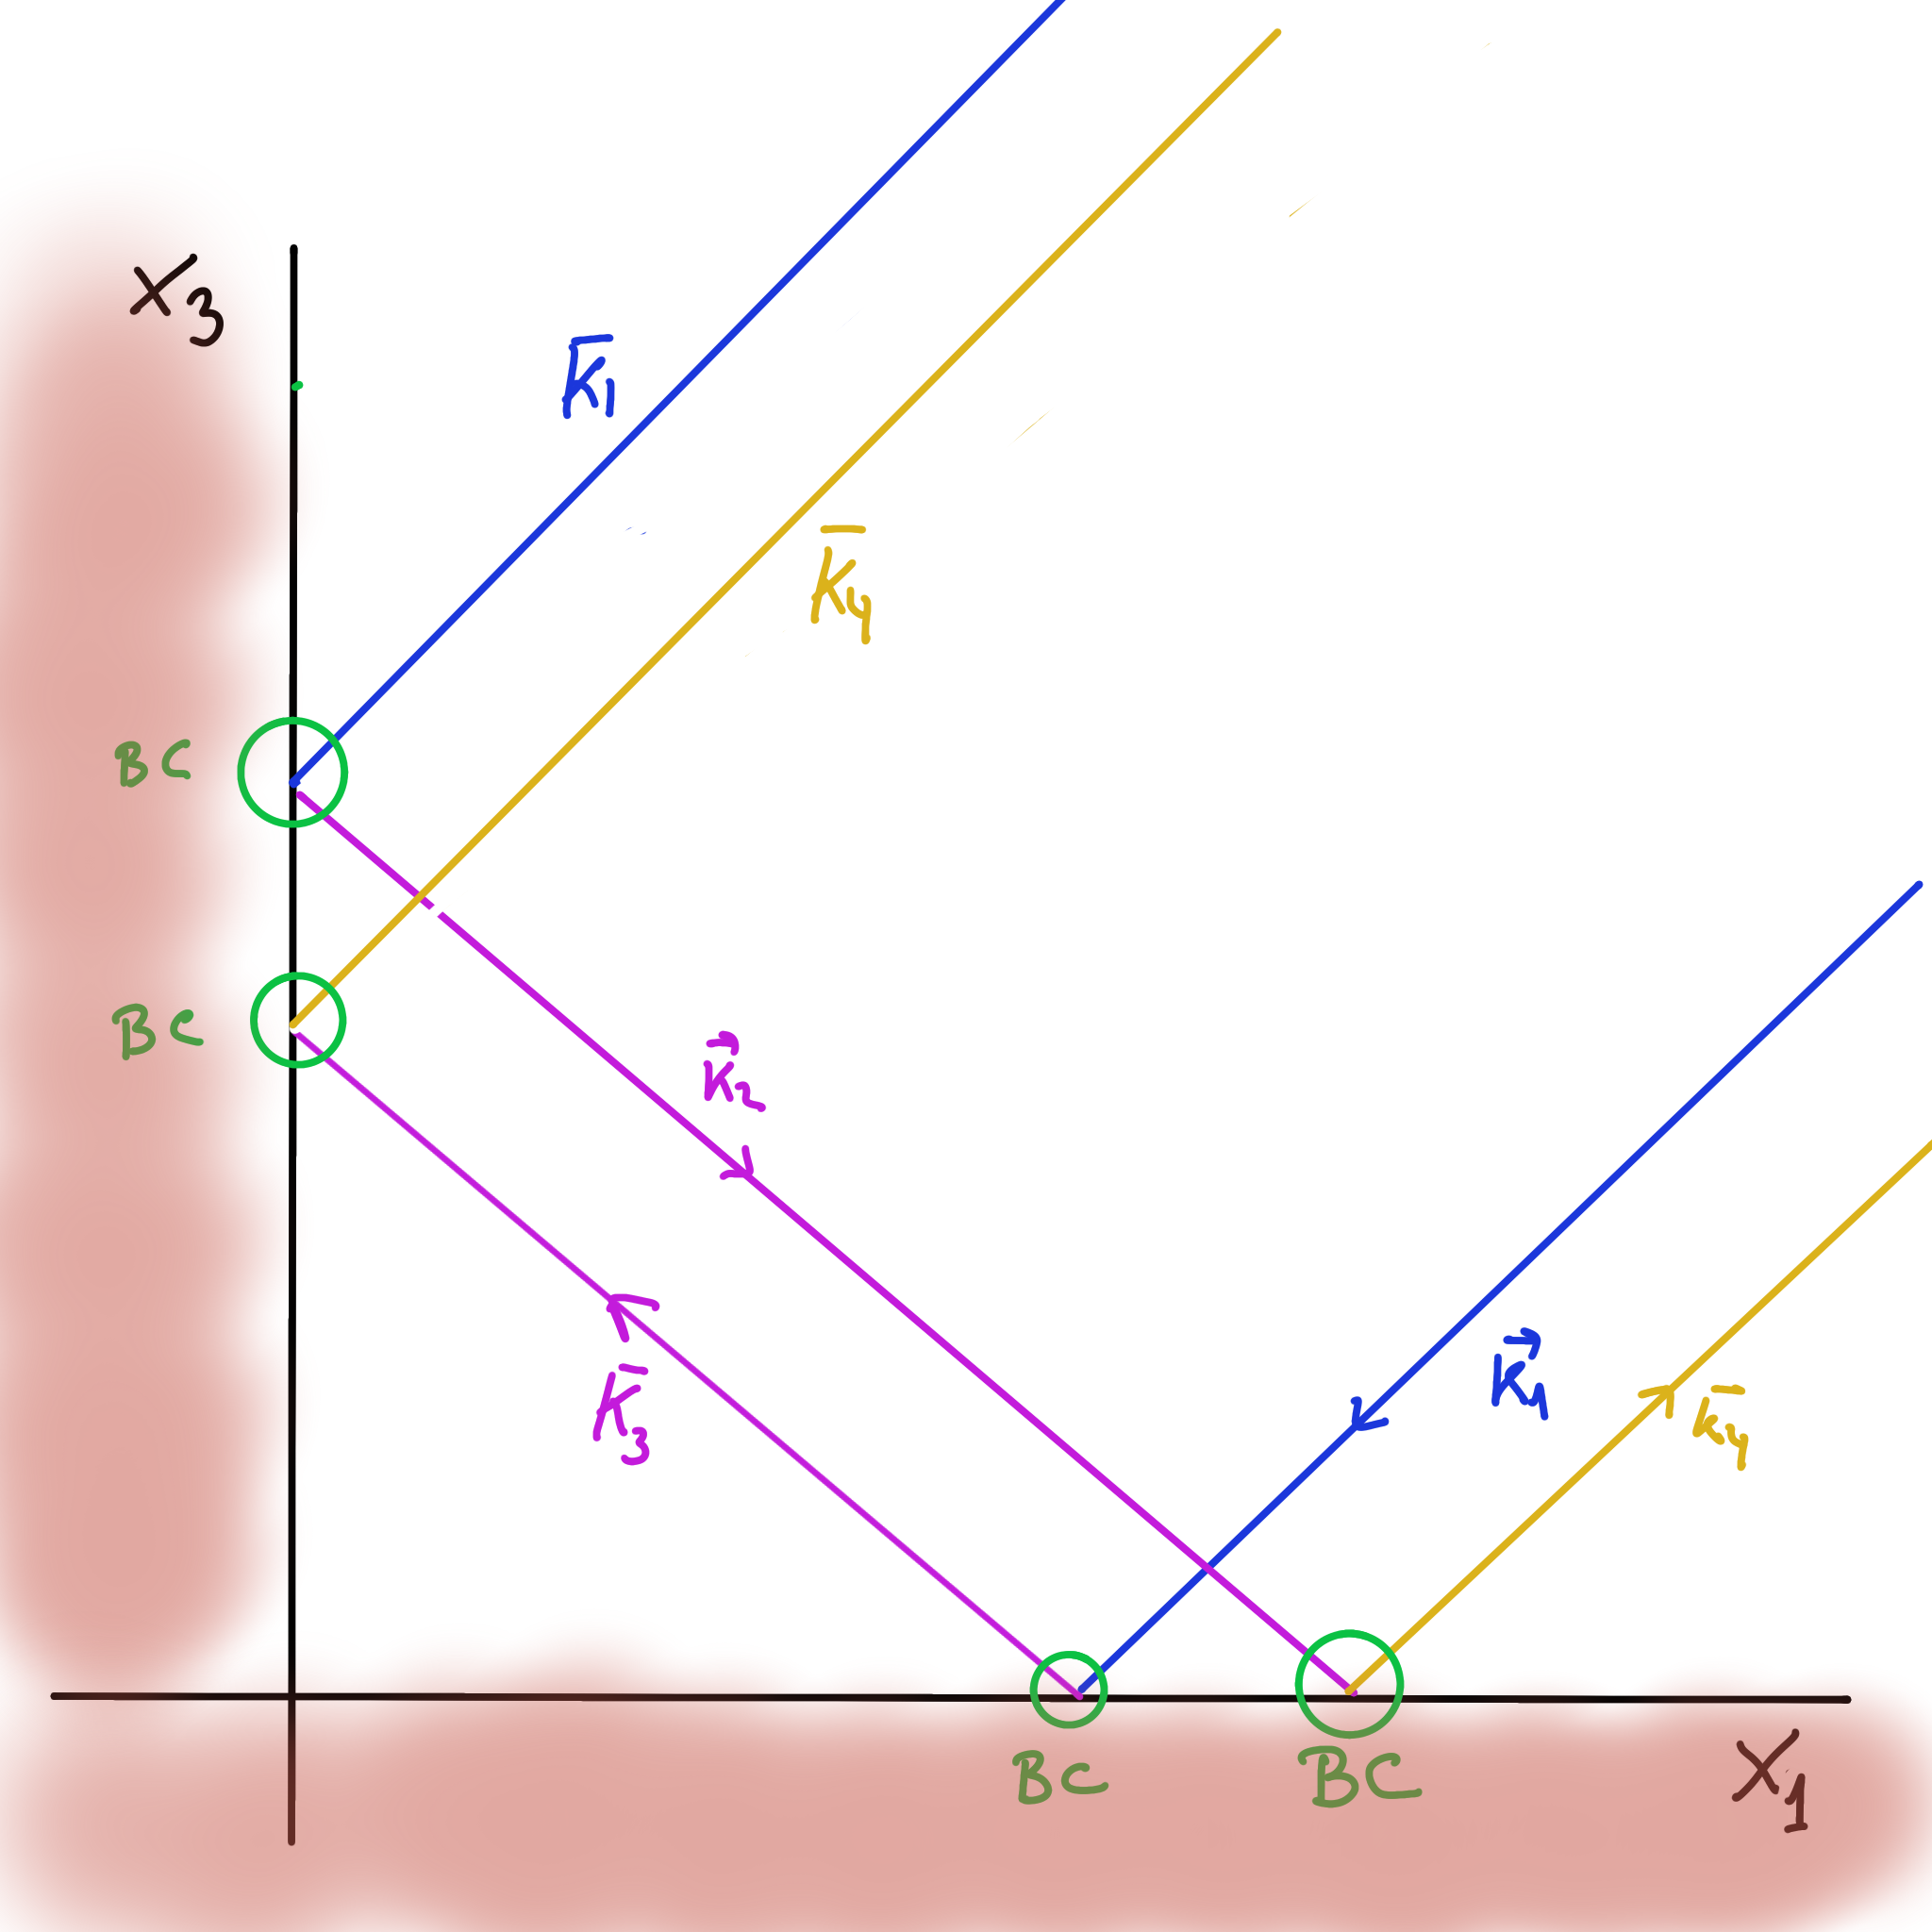
\includegraphics[width=6cm]{figures/X1x3plane.png}
	\centering
	\caption{Our bouncy wave.}
\end{figure}

Let us assume that $\mathbf{E}_{i}$ to be polarised in $\hat{x}_{2}$ direction. Their wave vectors have the following form:

\begin{equation}
	\mathbf{k}_{i} = \mp k_{1} \hat{x}_{1} \pm k_{3} \hat{x}_{3} + k_{2} \hat{x}_{2}.
\end{equation}

Now we have the crucial point; We will have to evaluate (\ref{eq:boundaryconditionsfields}) for \textit{each vertex}\footnote{Each vertex will be the LC of ingoing and outgoing waves respect to that plane.} in our system. This is:
		
		
\begin{equation}
	\begin{split}
		\left[\left(\mathbf{E}_{1} + \mathbf{E}_{2}\right) \times \hat{n} \right]_{x_{1}=0} &=0 \qquad \rightarrow \qquad E_{1} = - E_{2},\\
		\left[\left(\mathbf{E}_{3} + \mathbf{E}_{4}\right) \times \hat{n} \right]_{x_{1}=0} &=0 \qquad \rightarrow \qquad E_{3} = - E_{4},\\
		\left[\left(\mathbf{E}_{1} + \mathbf{E}_{3}\right) \times \hat{n} \right]_{x_{3}=0} &=0 \qquad \rightarrow \qquad E_{1} = - E_{3},\\
		\left[\left(\mathbf{E}_{3} + \mathbf{E}_{4}\right) \times \hat{n} \right]_{x_{3}=0} &=0 \qquad \rightarrow \qquad E_{2} = - E_{4}.
	\end{split}
\end{equation}

It is important to notice that $\hat{n}$ will be different depending on which surface we evaluate in. Previous results yields how the amplitudes are related for each wave. Putting that information together in the linear combination for these fields, we get:
	
\begin{equation}
	\begin{split}
		\mathbf{E}_{T} &= \sum_{i} \mathbf{E}_{i}, \\
		&= E_{0} \hat{x}_{2} \left(e^{i\left(-k_{1}x_{1} - k_{3}x_{3} \right)}
		-e^{i\left(k_{1}x_{1} - k_{3}x_{3} \right)}
		-e^{i\left(-k_{1}x_{1} +k_{3}x_{3} \right)}
		-e^{i\left(k_{1}x_{1} + k_{3}x_{3} \right)}\right) e^{i\left(k_{2}x_{2}-\omega t\right)},\\
		&= 4 E_{0} \hat{x}_{2} e^{i\left(k_{2}x_{2} - \omega t\right)} \sin\left(k_{1}x_{1}\right) \cos\left(k_{3}x_{3}\right).
	\end{split}
\end{equation}
		
\subsubsection{E: Waving at the Properties of a Wave}\label{E: Waving at the Properties of a Wave}
\textbf{\textcolor{red}{UNDER CONSTRUCTION}}
	


